\documentclass[oneside, astronomy, noacknowlegments]{BYUPhys}

% Your name
  \Author{Scott Leland Crossen}

% Enter the date your thesis is approved
  \Year{[Year]}
  \Month{[Approval Month]}

% If you have a long title, split it between multiple lines using the \\ command
  \Title{Optically Detected Magnetic Resonance;
Computational Predictions\\and Experimental Results
  }

% Your research advisor
\AdvisorTitle{Advisor}
  \Advisor{Dr. John S. Colton}

% For honors theses, enter the name of the honors Representative
  \HonorsRepresentative{Kristine Hansen}

% The text of your abstract
  \Abstract{ [The abstract is a summary of the thesis/dissertation
  with emphasis on the findings of the study. The abstract must not
  exceed 350 words in length and fit on one page, single spaced.] }

 \Keywords{[A comma-separated list of descriptive words for search purposes]}

% Acknowledge those who helped and supported you
  \Acknowledgments{
    [Acknowledgements should be simple, in good taste, and fit on one page]
  }

%% The members of your committee (masters only need A and B, PhD need all 4)
%  \MemberA{Committee Member A}
%  \MemberB{Committee Member B}
%  \MemberC{Committee Member C}
%  \MemberD{Committee Member D}
%

\begin{document}

 % Start page counting in roman numerals
 \frontmatter

 % This command makes the formal preliminary pages.
 % You can comment it out during the drafting process if you want to save paper.
 \makepreliminarypages

 % Make the table of contents.
 \tableofcontents

 % Start regular page counting at page 1
 \mainmatter

% OK. Everything is set up. Type your thesis here.



\chapter{Introduction}

\section{Qualitative Description}
\label{sec:qualitative}

\textit{Optically Detected Magnetic Resonance} (ODMR) is a particular form of \textit{Electron Paramagnetic Resonance} (EPR) which is more commonly known as \textit{Electron Spin Resonance} (ESR). The latter two of these terms (EPR and ESR) are synonymous; The former (ODMR) is a particular subset of ESR that utilizes a luminescence measuring technique as a means to collect ESR information. In literature, it is common to see both of these terms followed by the designation "spectroscopy" - as that is what they are: tools to study properties of matter via electromagnetic radiation. Though the extent of their application has grown over the years, EPR and ODMR are most commonly used to study the spin-properties of electrons and electron-holes trapped in metal lattices. They can be used to study free radicals in organic materials and are also important in studying the local environment of lattice defects through a technique using angular-dependent ODMR. One particular use of ODMR is the study of electron-spin coherence via a technique known as \textit{Electron Spin Echo}. This can be useful when studying what properties and conditions lead to superior state coherence for qubit candidate materials in quantum computing.

The intellectual foundation of Electron Spin Resonance is rooted in Quantum Mechanics. Bound electrons in matter have discrete and quantized energy levels that govern what frequencies of light are emitted when transitions between energy levels are made. For electron systems, which are fermions and thus subject to the Pauli exclusion principle, the energy levels are 2nd order degenerate when bound in matter. In Quantum Mechanics we choose to describe this degeneracy in terms of spins: we say an electron is either "spin-up" or "spin-down". Each energy level can have at most two electrons of opposite spins inhabiting it (and thus the degeneracy). The spin terminology is moot however, and is really just an attempt to describe electrons as particles - which may be useful for neophytes attempting to learn the material but for our purposes may only confuse the reader to view reality in this way. Furthermore, "electron spin" is a meaningless term unless the "particle" is in the presence of a magnetic field. In this case the energy levels of the molecule will split according to the "zeeman effect" and the spin-states of the electrons can be observed - most commonly through a photoluminescence technique.

Moreover, In the presence of a magnetic field, populations of free electrons will form a spin-1/2 system between a higher-energy "spin-up" state and a lower-energy "spin-down" state. In matter, different parities of spin-states can be formed between the interactions of different energy levels with different transition selection-rules. For a given magnetic-field strength there will be a set of characteristic microwave frequencies that the electrons emit when transitioning between these quantized states. Likewise, for a given microwave target signal, there will be a variety of magnetic field strengths which are most adept at transitioning bound electrons between states. This unique pairing between both the microwave frequency and magnetic field strength is what ESR Spectroscopy essentially is and what it uses to discover information about materials.







\chapter{A Sample Chapter}

\section{A Fascinating Section}
\label{sec:meaningfulname}

For a short thesis, you can usually just type the whole body of the
thesis here.  For longer documents you might consider typing
chapters in separate files and using the \verb|\include| command.
There is another example on the physics web page
(\href{http://www.physics.byu.edu/undergraduate/latex.aspx}{click
here to go there}) that shows how to do this.

You can create your bibliography right in the main tex document.
Here are references to a book \cite{Jackson1998}, an article
\cite{Peatross2000}, and a web site \cite{intel}. You can also use
BibTeX to keep track of your references.  The method for using
BibTeX is shown in the other example on the physics web page.

Making an index is easy. Just use the \verb|\index{Key}| command.
\index{Index!Making} You can include figures too (see
Fig.~\ref{fig:MirrorDiagram}).  Usually you need both eps and pdf
versions of each figure.
\begin{figure}
    \centerline{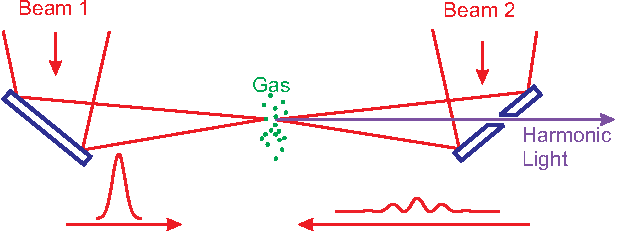
\includegraphics{Graphic1}}
    \caption[Setup for using counter-propagating light]{\label{fig:MirrorDiagram}
    A mirror with a hole is used to extract high-order harmonics generated in
    counter-propagating laser beams.}
\end{figure}

% Start labeling chapters with letters and calling them appendices
\begin{appendices}

\chapter{Appendix Title}
\label{sec:appendixname}

You can put supplimentary content in an appendix.

\end{appendices}

% Make the bibliography.
% Enter your references in the BibTex file "references.bib"
 \bibliography{references}

% Make the index
 \printindex

\end{document}
